\documentclass[11pt,a4paper]{article}
\usepackage{fontspec}
\usepackage{unicode-math}
\usepackage{libertineotf}
\usepackage{tikz}
\usepackage{csquotes}
\newcommand{\package}[1]{\emph{#1}}
\begin{document}
\title{Page layout with \package{reledpar}}
\author{Dominico Cufalo and Maïeul Rouquette}
\date{August 17, 2017}
\maketitle
\begin{figure}[p]\centering
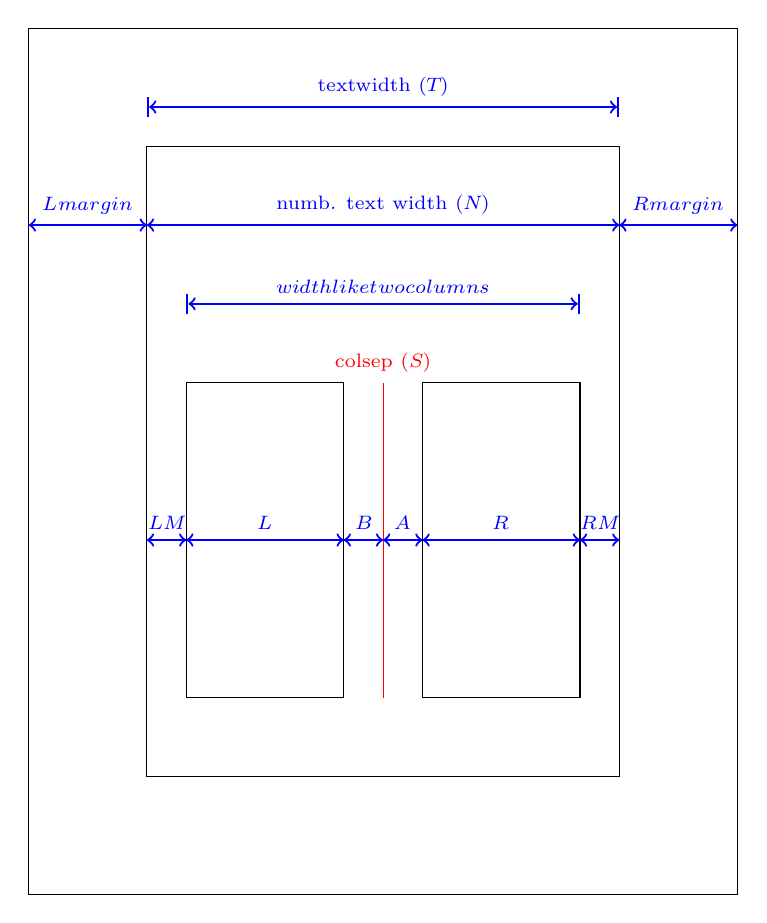
\begin{tikzpicture}[every node/.style={anchor=above,font=\scriptsize}]
	\draw (0,0) rectangle (6,8);
	\draw (-1.5,-1.5) rectangle (7.5,9.5);
	\draw (0.5,1) rectangle (2.5,5);
	\draw (3.5,1) rectangle (5.5,5);
	\draw[blue,thick,|<->|] (0,8.5) -- node[above] {textwidth ($T$)} (6,8.5);
	\draw[blue,thick,<->] (-1.5,7) -- node[above] {$Lmargin$} (0,7);
	\draw[blue,thick,<->] (0,7) -- node[above] {numb. text width ($N$)} (6,7);
	\draw[blue,thick,<->] (6,7) -- node[above] {$Rmargin$} (7.5,7);
	\draw[blue,thick,|<->|]  (0.5,6) -- node[above] {$widthliketwocolumns$} (5.5,6);
	\draw[red] (3,1) -- (3,5) node[above] {colsep ($S$)};
	\draw[blue,thick,<->] (0,3) -- node[above] {$LM$} (0.5,3);
	\draw[blue,thick,<->] (0.5,3) -- node[above] {$L$} (2.5,3);
	\draw[blue,thick,<->] (2.5,3) -- node[above] {$B$} (3,3);
	\draw[blue,thick,<->] (3,3) -- node[above] {$A$} (3.5,3);
	\draw[blue,thick,<->] (3.5,3) -- node[above] {$R$} (5.5,3);
	\draw[blue,thick,<->] (5.5,3) -- node[above] {$RM$} (6,3);
\end{tikzpicture}
\caption{Page layout}\label{pic:page}
\end{figure}
\section{General}
\package{Reledmac} doesn't care neither text width ($T$) nor margins, whose sizes are calculated by \LaTeX{} itself or depends on other packages like \package{geometry}. In normal typesetting, line numbers and sidenotes are in the margin.

In parallel typesetting, sidenotes and lines numbers can be, or not, in page margins. 

Normally, we get:

\begin{equation}
  T = LM + L + B + S + A + R + RM
\end{equation}

The only possible exceptions occur when the user makes mistakes when fixing $L$ and / or $A$ and / or $B$ and / or $R$.
\section{Parameters}
Now, let's turn our attention to the the parameters that can be controlled by \package{reledmac} are (see fig.~\ref{pic:page}). These are:

\begin{description}	
	\item[N] The numbered text width, \emph{i. e.} the width of text with line numbers. Its width is by default equal to $T$, but can be also modified by the \package{reledmac!}\package{reledpar} option \verb!widthliketwocolumns!: in this case, $N=L+B+S+A+R$
	
	\item[L] \verb!\Lcolwidth!; fixed width, by default \verb!{0.45\textwidth}!
	
	\item[R] \verb!\Rcolwidth!; fixed width, by default \verb!{0.45\textwidth}!
	
	\item[S] \verb!\columnseparator!; it inserts a vertical rule of width \verb!\columnrulewidth!, by default set to be $0\,pt$. You can redefine \verb!\columnrulewidth! by
	
\begin{verbatim}
	\setlength{\columnrulewidth}{0.4pt}
\end{verbatim}
	
	\item[B] \verb!\beforecolumnseparator!: automatically calculated, but can be redefined by
	
\begin{verbatim}
	\setlength{\beforecolumnseparator}{<length>}
\end{verbatim}
	
	\item[A] \verb!\aftercolumnseparator!: automatically calculated, but can be redefined by

\begin{verbatim}
	\setlength{\aftercolumnseparator}{<length>}
\end{verbatim}

\end{description}

\section{Columns' position}
By default, columns are positioned to the right of the page. However, you can use
\verb!\columnsposition{L}! to align them to the left, or \verb!\columnsposition{C}! to center
them.

In this case $LM$ and $RM$ are modified according:

\begin{itemize}
	\item with \verb!\columnsposition{L}!, $LM=0$ and $RM$ is automatically calculated
	\item with \verb!\columnsposition{R}!, $RM=0$ and $LM$ is automatically calculated
	\item with \verb!\columnsposition{C}!, $RM$ and $LM$ are automatically calculated
\end{itemize}

\section{Automatically calculated parameters}
Therefore, the length automatically calculated are $LM$, $RM$, and, if not fixed by user, $B$ and $A$. 


\subsection{If $LM$, $RM$, $B$ and $A$ are calculated}
\begin{equation}
	LM = RM = B = A = \frac{T - (L + S + R)}{4}
\end{equation}

\subsection{If $LM$, $RM$, $B$ are calculated}

\begin{equation}
	LM = RM = B = \frac{T - (L + A + S + R)}{3}
\end{equation}

\subsection{If $LM$, $RM$, $A$ are calculated}

\begin{equation}
	LM = RM = A = \frac{T - (L + B + S + R)}{3}
\end{equation}
\subsection{If only $LM$ and $RM$ are concerned}

\begin{equation}
	LM = RM = \frac{T - (L + B + S + A + R)}{2}
\end{equation}

\subsection{In any case}
$LM$, $B$, $A$, $RM$ can't have a negative value. If the result of one the previous equation is negative, then that means the value equals to $0$.

Technically, the \enquote{calculated values} are determined using \verb+\hfill+.

\end{document}
